% SECTION ====================================================================================
\vspace{-4pt}
\begin{sectionbox}
\section{Graphen}
% ============================================================================================
\subsection{Terminologie}\smallskip
Ein Graph $G=(V,E)$ besteht aus der Menge von Kanten $V=\{v_{1},\ldots,v_{1^n}\}$ und der Menge von Kanten $E$.\par\smallskip
\end{sectionbox}
\vspace{-4pt}
\begin{sectionbox}
\textbf{Gerichteter Graph}: $E \subseteq V \times V=\{(u, v): u \in V, v \in V\}$\par
\begin{itemize}
    \item $w \in V$ heisst \textbf{adjazent} zu $v \in V$, falls $(v, w) \in E$
    \item Vorgänger eines Knotens $v$: $N^{-}(v):=\{u \in V |(u, v) \in E\}$
    \item Nachfolger eines Knotens $v$: $N^{+}(v):=\{u \in V |(v, u) \in E\}$
    \item Eingangsgrad: $\operatorname{deg}^{-}(v):=|N^{-}(v)|$
    \item Ausgangsgrad: $\operatorname{deg}^{+}(v):=|N^{+}(v)|$
\end{itemize}\par\smallskip
\begin{center}
    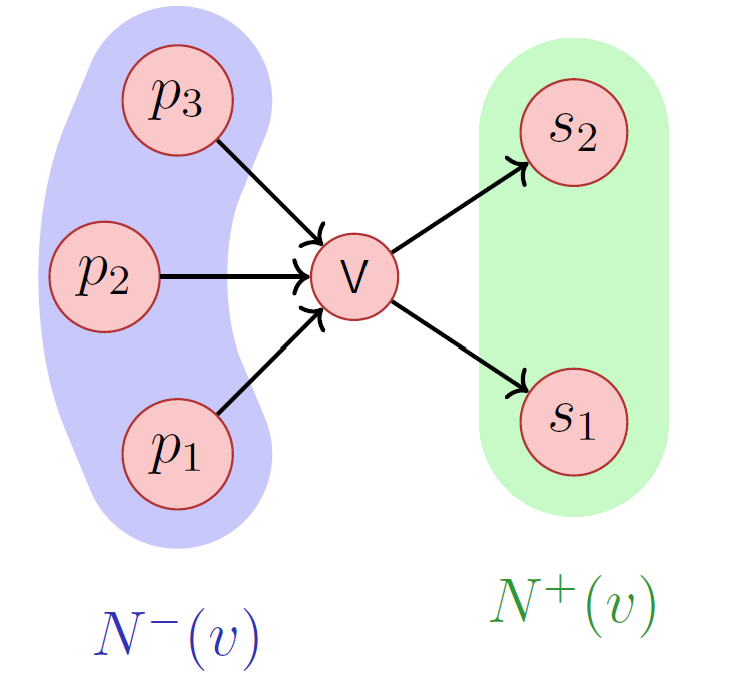
\includegraphics[width=0.5\columnwidth]{../img/gerGraph.png}
\end{center}\par\smallskip
\end{sectionbox}
\vspace{-4pt}
\begin{sectionbox}
\textbf{Ungerichteter Graph}: $E \subseteq \{(u, v): v \in V, u \in V\}$\par
\begin{itemize}
    \item $w \in V$ heisst \textbf{adjazent} zu $v \in V$, falls $\{v, w\} \in E$
    \item Nachbarschaft: $N(v):=\{w \in V |\{v, w\} \in E\}$
    \item Grad: $\operatorname{deg}(v):=|N(v)|$ (Schleifen zählen 2)
\end{itemize}\par\smallskip

\end{sectionbox}
\vspace{-4pt}
\begin{sectionbox}

\textbf{Vollständiger Graph}: Ungerichteter Graph mit  $E=\{(u, v): u \in V, v \in V, \quad c \neq v\}$\par\smallskip
\textbf{Bipartiter Graph}: Graph, bei dem $V$ so in disjunkte $U$ und $W$ aufgeteilt werden kann, dass alle $e \in E$ einen Knoten in $U$ und einen in $W$ haben\par
%\begin{center}
%   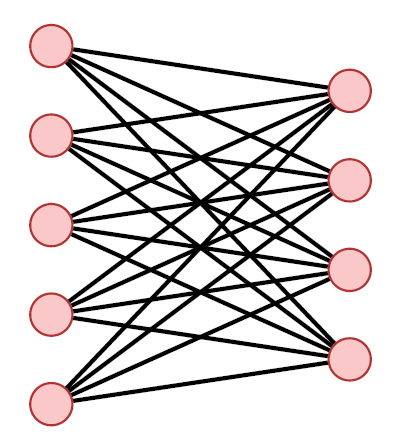
\includegraphics[width=0.25\columnwidth]{../img/biparGraph.png}
%\end{center}\par\smallskip
\end{sectionbox}
\vspace{-4pt}
\begin{sectionbox}
\textbf{Handschlag-Lemma:}
\begin{itemize}
    \item $\sum_{v \in V}\limits \text{deg}^- (v) = \sum_{v \in V} \text{deg}^+ (v) = |E|$, falls $G$ gerichtet
    \item $\sum_{v \in V}\limits \text{deg} (v) = 2 |E|$, falls $G$ ungerichtet
\end{itemize}
\end{sectionbox}
\vspace{-4pt}
\begin{sectionbox}
\textbf{Wege}:\par
\begin{itemize}
    \item \textbf{Weg / Path}: Sequenz von Knoten $p=\left\langle v_{1}, v_{2}, \ldots, v_{k}\right\rangle$ so dass für jedes $i \in\{1 \ldots k\}$ eine Kante von $v_{i}$ nach $v_{i+1}$ existiert
    \item \textbf{Pfad / einfacher Pfad / simple path}: Weg der keinen Knoten mehrfach verwendet
    \item \textbf{Länge des Weges}: Anzahl enthaltene Kanten $k$
    \item \textbf{Gewicht des Weges} (in gewichteten Graphen): $\sum_{i=1}^{k} c\left(\left(v_{i}, v_{i+1}\right)\right)$ (bzw. $\left.\sum_{i=1}^{k} c\left(\left\{v_{i}, v_{i+1}\right\}\right)\right)$
\end{itemize}\par\smallskip

\end{sectionbox}
\vspace{-4pt}
\begin{sectionbox}
\textbf{Zusammenhang}:\par
\begin{itemize}
    \item Ungerichteter Graph heisst \textbf{zusammenhängend}, wenn für jedes Paar $v, w \in V$ ein verbindender Weg existiert.
    \item Gerichteter Graph heisst \textbf{stark zusammenhängend}, wenn für jedes Paar $v, w \in V$ ein verbindender Weg existiert.
    \item Gerichteter Graph heisst \textbf{schwach zusammenhängend}, wenn der entsprechende ungerichtete Graph zusammenhängend ist.
\end{itemize}\par\smallskip

\end{sectionbox}
\vspace{-4pt}
\begin{sectionbox}
\textbf{Zyklen}:\par
\begin{itemize}
    \item \textbf{Zyklus}: Weg (und nicht einfacher Pfad!) $\left\langle v_{1}, \ldots, v_{k+1}\right\rangle$ mit $v_{1}=v_{k+1}$
    \item \textbf{Einfacher Zyklus}: Zyklus, aber Knoten kommen nicht mehrfach vor (ausser $s$ und $t$)
    \item \textbf{Kreis}: Zyklus mit paarweise verschiedenen $v_{1}, \ldots, v_{k},$ welcher keine Kante mehrfach verwendet
    \item \textbf{Kreisfrei (azyklisch)}: Graph ohne jegliche Kreise.
\end{itemize}\par

\end{sectionbox}
\vspace{-4pt}
\begin{sectionbox}
\textbf{Beobachtungen}\par
\begin{itemize}
    \item Allgemein: $0 \leq|E| \in \mathcal{O}\left(|V|^{2}\right)$
    \item Zusammenhängender Graph: $|E| \in \Omega(|V|)$
    \item Vollständiger Graph: $|E|=\frac{|V| \cdot(|V|-1)}{2}$ (ungerichtet)
    \item Maximal $|E|=|V|^{2}(\text { gerichtet })$
    \item Maximal $|E|=\frac{|V| \cdot(|V|+1)}{2}$ (ungerichtet)
\end{itemize}\par\smallskip
\end{sectionbox}

\vspace{-4pt}
\begin{sectionbox}
\subsection{Repräsentation von Graphen}\smallskip

\subsubsection{Adjazenzmatrix}\par\smallskip
Graph $G=(V, E)$ mit Knotenmenge $v_{1}, \ldots, v_{n}$ gespeichert als Adjazenzmatrix $A_{G}=\left(a_{i j}\right)_{1 \leq i, j \leq n}$ mit Einträgen aus $\{0,1\}$. $a_{i j}=1$ genau dann wenn Kante von $v_{i}$ nach $v_{j}$. Speicherbedarf $\Theta\left(|V|^{2}\right)$. $A_{G}$ ist symmetrisch, wenn $G$ ungerichtet.\par\smallskip
\begin{center}
    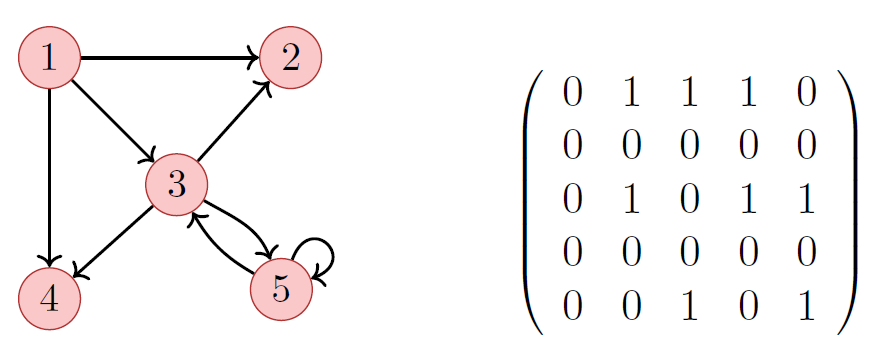
\includegraphics[width = 0.9\columnwidth]{../img/AdjMa.png}
\end{center}
\end{sectionbox}

\vspace{-4pt}
\begin{sectionbox}
\subsubsection{Adjazenzliste}\par\smallskip
Viele Graphen $G=(V, E)$ mit Knotenmenge $v_{1}, \ldots, v_{n}$ haben deutlich weniger als $n^{2}$ Kanten. Repräsentation mit Adjazenzliste: Array $A[1], \ldots, A[n]$, $A_{i}$ enthält verkettete Liste aller Knoten in $N^{+}\left(v_{i}\right)$. Speicherbedarf $\Theta\left(|V|+|E|\right)$.\par\smallskip
\begin{center}
    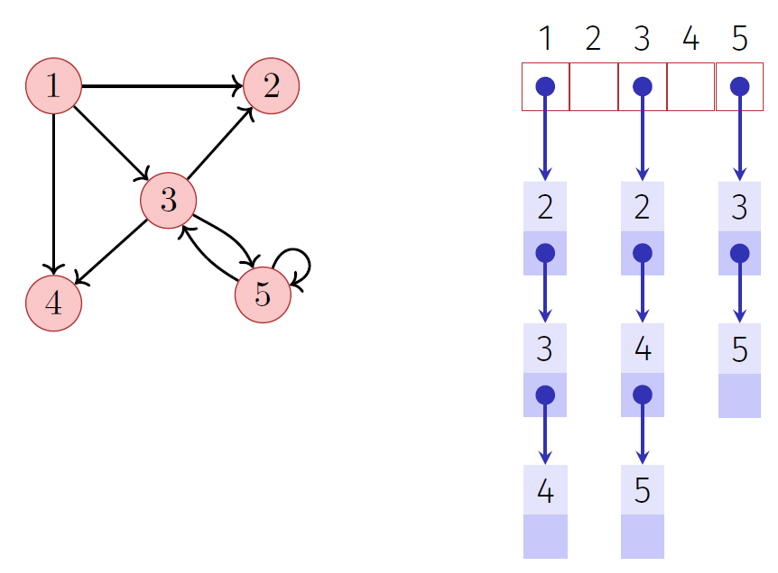
\includegraphics[width = 0.9\columnwidth]{../img/AdjList.png}
\end{center}

\subsubsection{Laufzeiten einfacher Operationen}\par\smallskip
\begin{center}
    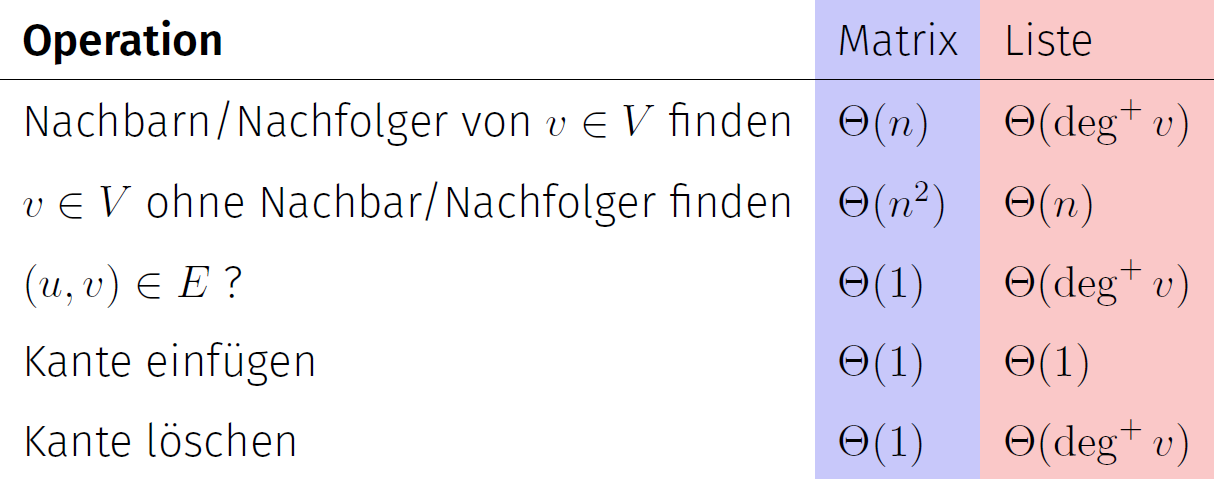
\includegraphics[width = \columnwidth]{../img/AdjLaufzeiten.png}
\end{center}\smallskip
\end{sectionbox}
\vspace{-4pt}
\begin{sectionbox}
\subsection{Graphen Traversieren: Tiefensuche}\smallskip
Verfolge zuerst Pfad in die Tiefe, bis nichts mehr besucht werden kann.\par
\begin{center}
    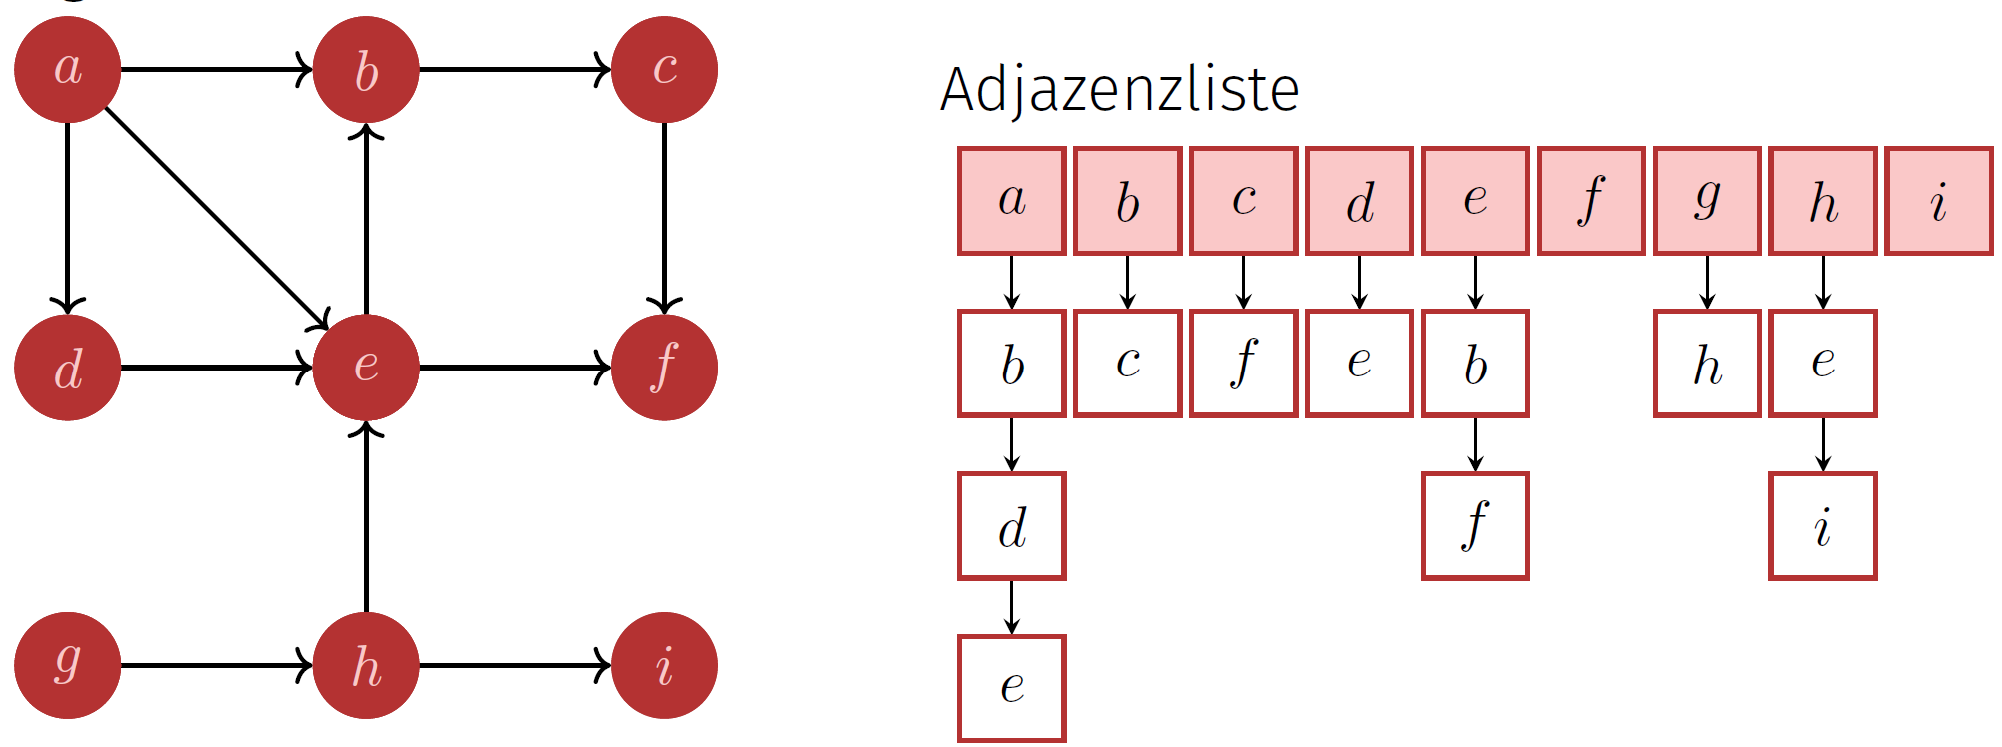
\includegraphics[width = 0.9\columnwidth]{../img/DFS_sym.png}
\end{center}\par
Reihenfolge: $a, b, c, f, d, e, g, h, i$\medskip

\textbf{Tiefensuche ab Knoten $v$: DFS-Visit(G,v)}\par
Laufzeit (ohne Rekursion): $\Theta\left(\operatorname{deg}^{+} v\right)$\par\smallskip

\textbf{Tiefensuche für alle Knoten: DFS-Visit(G)}\par
Laufzeit: $\Theta(|V|+\sum_{v \in V}(\operatorname{deg}^{+}(v)+1))=\Theta(|V|+|E|)$\par\smallskip

\begin{tabular*}{\columnwidth}{@{\extracolsep\fill}ll@{}}
\textbf{DFS-Visit(G,v)} & \textbf{DFS-Visit(G)} \\
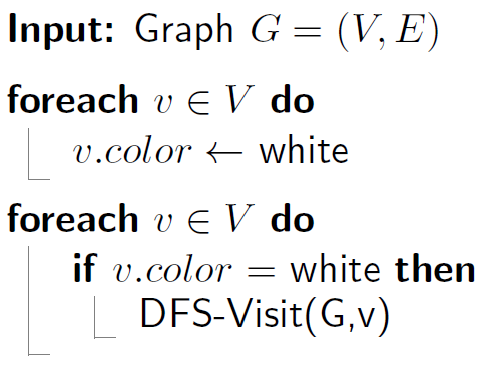
\includegraphics[width = 0.40\columnwidth]{../img/DFSG.png} &
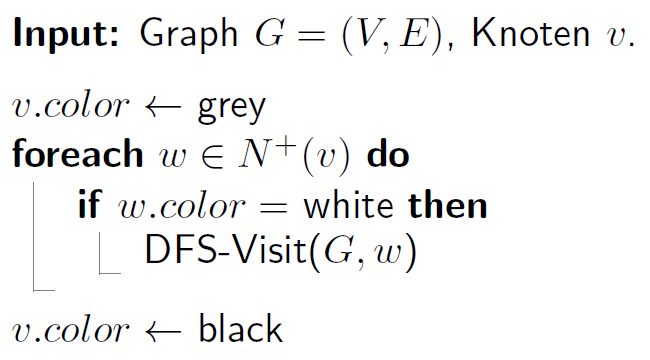
\includegraphics[width = 0.54\columnwidth]{../img/DFSGv.png} \\
\end{tabular*}\smallskip
\end{sectionbox}
\vspace{-4pt}
\begin{sectionbox}
\subsection{Graphen Traversieren: Breitensuche}\smallskip
Verfolge zuerst Pfad in die Breite, gehe dann in die Tiefe.\par
\begin{center}
    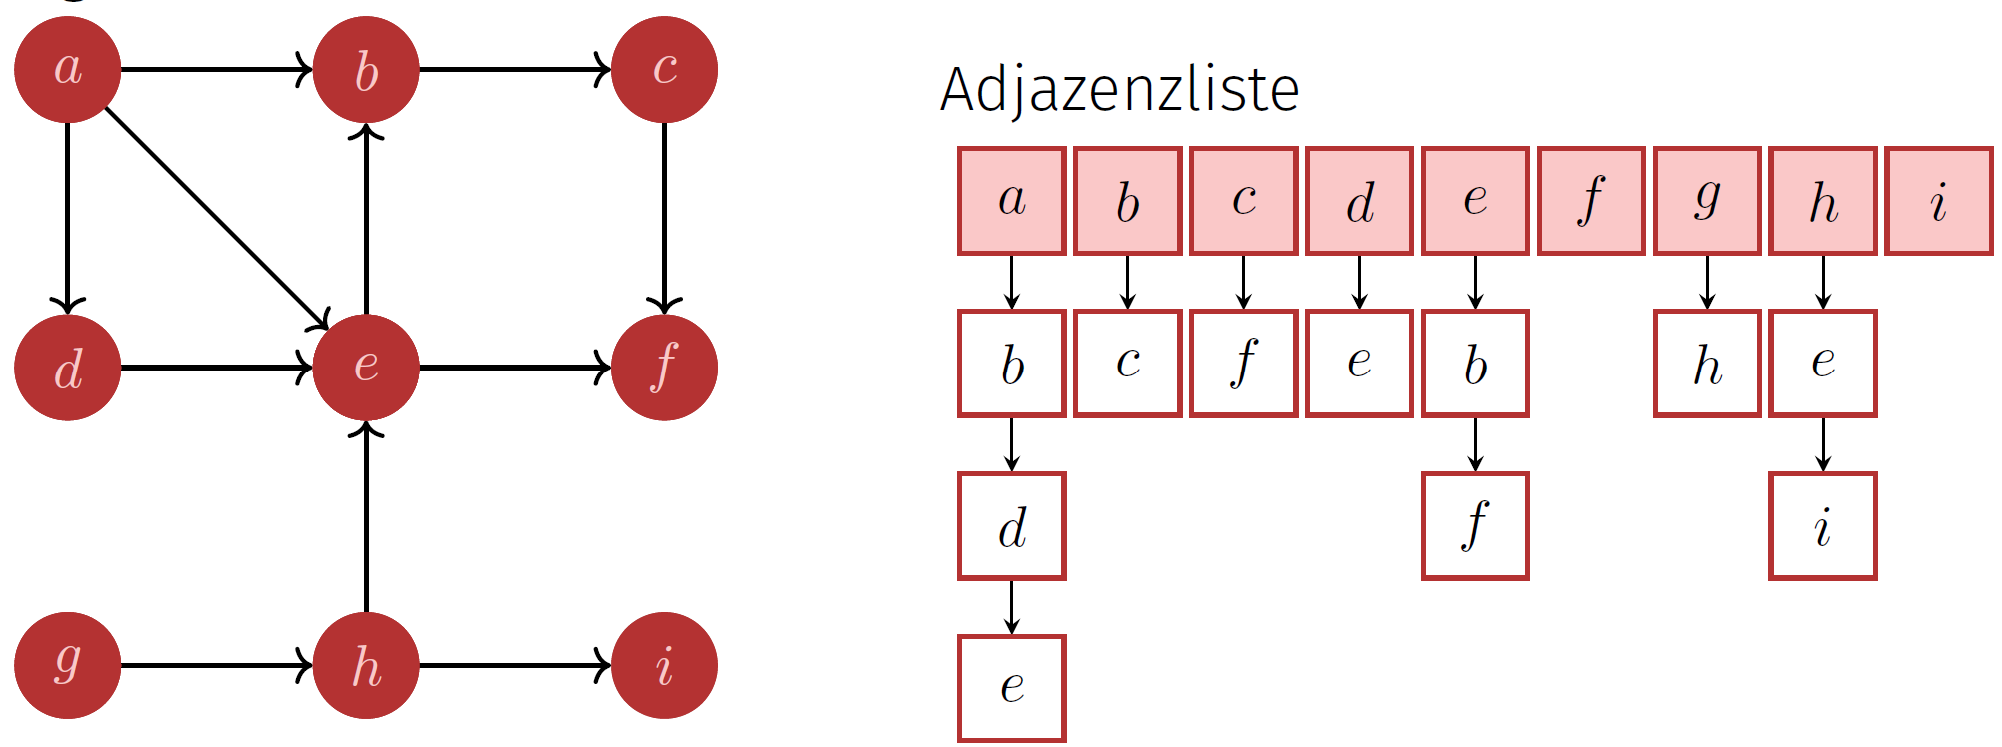
\includegraphics[width = 0.9\columnwidth]{../img/DFS_sym.png}
\end{center}\par
Reihenfolge: $a, b, d, e, c, f, g, h, i$\medskip

\begin{tabular*}{\columnwidth}{@{\extracolsep\fill}ll@{}}
\textbf{BFS-Visit(G,v)} & $\quad \quad \quad \quad$\textbf{BFS-Visit(G)} \\
\multicolumn{2}{l}{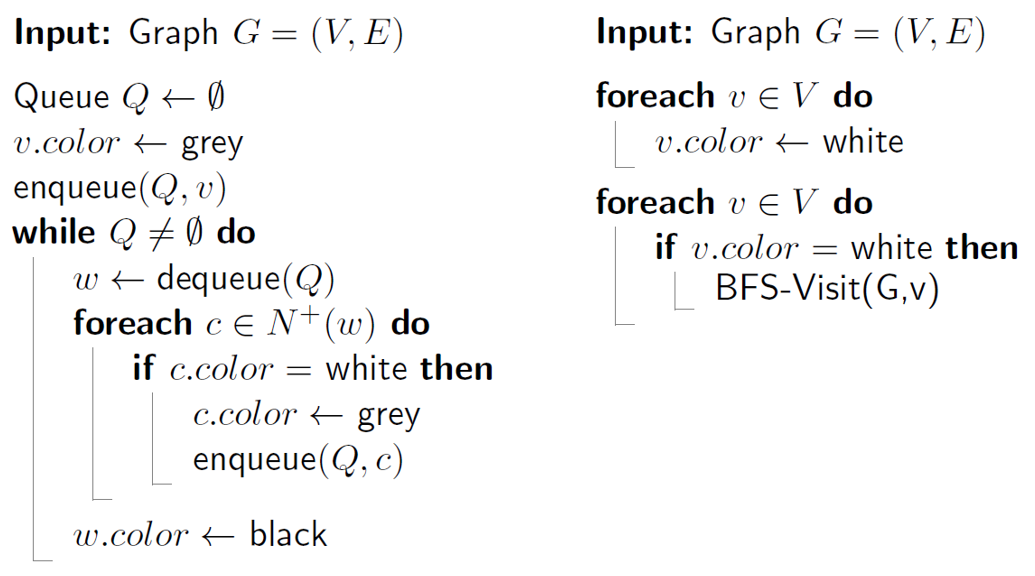
\includegraphics[width = 0.9\columnwidth]{../img/BFS.png}} \\
Extraplatz: $\mathcal{O}(|V|)$&  $\quad \quad \quad \quad$ Laufzeit: $\Theta(|V|+|E|)$ \\
\end{tabular*}

\end{sectionbox}
\vspace{-4pt}
\begin{sectionbox}
\subsection{Topologische Sortierung}\smallskip
\begin{greenbox}
Ein gerichteter Graph $G=(V, E)$ besitzt genau dann eine topologische Sortierung, wenn er \textbf{kreisfrei} ist.
\end{greenbox}\smallskip

\begin{center}
    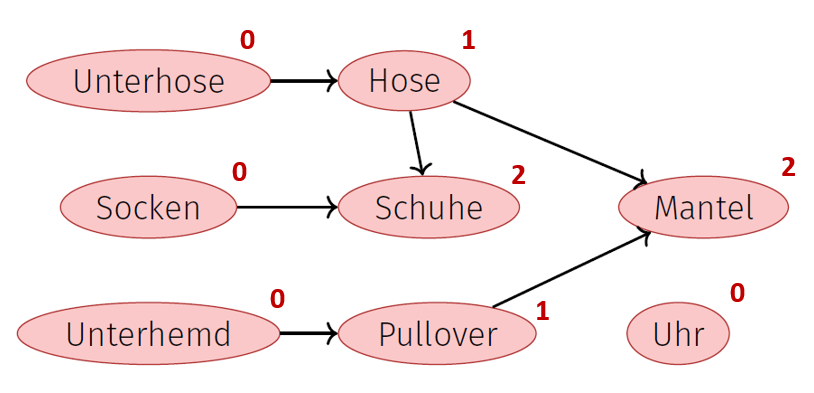
\includegraphics[width = 0.9\columnwidth]{../img/topoSort.png}
\end{center}\par\smallskip
Augmentiere den Eingangsgrad. Abbarbeitung nur wenn Eingangsgrad $0$ ist. Eingangsgrad verringern entspricht Knotenentfernen.\par\smallskip

\textbf{Topological-Sort(G)}\par
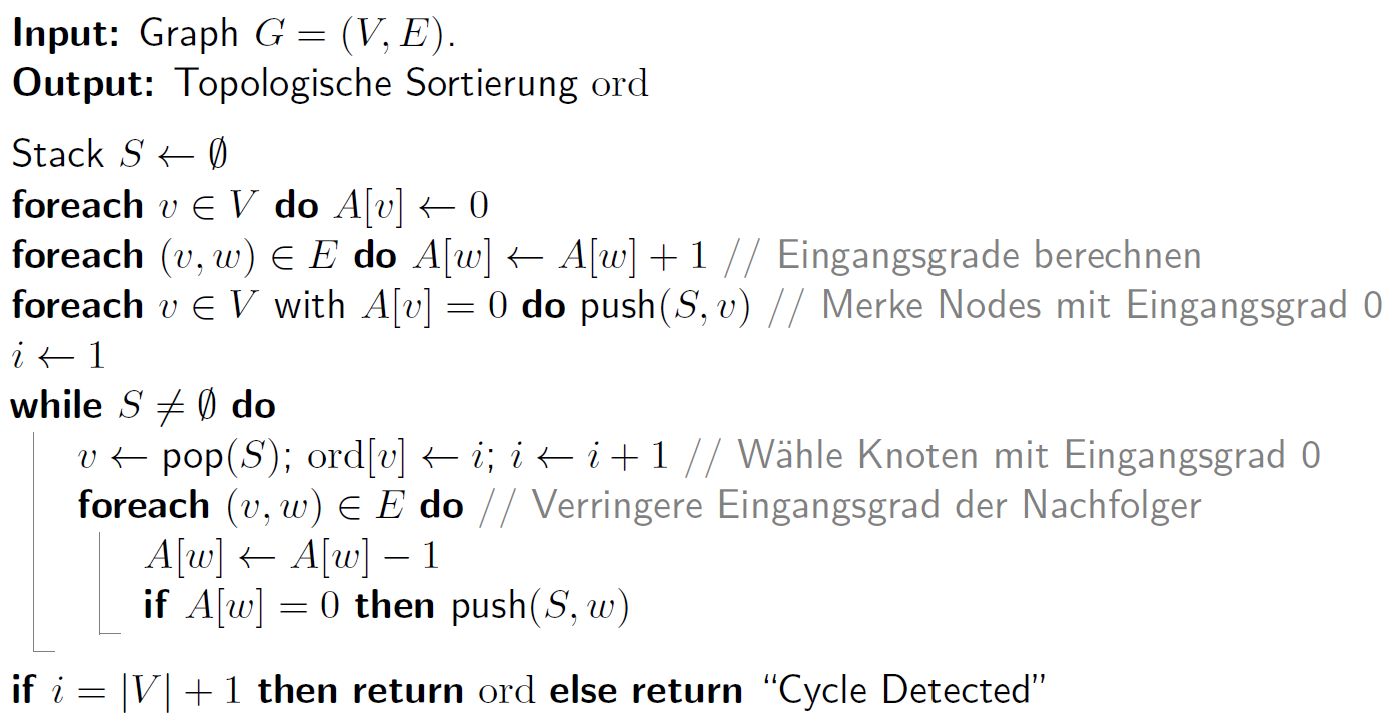
\includegraphics[width = \columnwidth]{../img/topoSortG.png}\par\smallskip

\textbf{Analyse}\par
\begin{itemize}
    \item Sei $G=(V, E)$ ein gerichteter, kreisfreier Graph. Der Algorithmus Topological-Sort berechnet in Zeit $\Theta(|V|+|E|)$ eine topologische Sortierung $\operatorname{ord}$ für $G$.
    \item Sei $G=(V, E)$ ein gerichteter, \textbf{nicht}-kreisfreier Graph. Der Algorithmus Topological-Sort terminiert in Zeit $\Theta(|V|+|E|)$ und detektiert den Zyklus.
\end{itemize}

\end{sectionbox}
\vspace{-4pt}
\begin{sectionbox}
\subsection{Kürzeste Wege}\smallskip
\textbf{Notation}\par\smallskip
$\delta(u, v)=$ Gewicht eines kürzesten Weges von $u$ nach $v$\par
$\delta(u, v)=\left\{\begin{array}{ll}
\infty & \text { kein Weg von } u \text { nach } v \\
\min \{c(p): u \stackrel{p}{\longrightarrow} v\} & \text { sonst }
\end{array}\right.$\par\smallskip

\textbf{Beobachtungen}\par
\begin{itemize}
    \item Einfachster Fall: Kantengewicht 1 $\rightarrow$ Breitensuche
    \item Es gibt Situationen, in denen kein kürzester Weg existiert: negative Zyklen könnten auftreten.
    \item Es kann exponentiell viele Wege geben $\rightarrow$  alle Wege probieren ist ineffizient
    \item Ein kürzester Weg von $s$ nach $v$ (ohne weitere Einschränkungen) kann nicht länger sein als ein kürzester Weg von $s$ nach $v$, der $u$ enthalten muss.\par
    \textcolor{tanne}{\textbf{$\delta(s, v) \leq \delta(s, u)+\delta(u, v)$}}
    \item \textbf{Optimale Substruktur}: Teilpfade von kürzesten Pfaden sind kürzeste Pfade ( \textbf{\textcolor{tanne}{Kürzester Pfad $\Rightarrow$ kürzeste Subpfäde}} )
    \item Kürzeste Wege enthalten keine Zyklen
\end{itemize}\par
\end{sectionbox}
\vspace{-4pt}
\begin{sectionbox}
\subsubsection{Allgemeiner Algorithmus (Relaxier-Algorithmus)}\smallskip
Gesucht: Kürzeste Wege von einem Startknoten $s$ aus.
\begin{itemize}
    \item Gewicht des kürzesten bisher gefundenen Pfades
    \begin{itemize}
        \item Zu Beginn: $d_{s}[v]=\infty$ für alle Knoten $v \in V$
        \item Ziel: $d_{s}[v]=\delta(s, v)$ für alle $v \in V$
    \end{itemize}
    \item Vorgänger eines Knotens: u Beginn $\pi_{s}[v]$ undefiniert für jeden Knoten $v \in V$
\end{itemize}\smallskip
\end{sectionbox}
\vspace{-4pt}
\begin{sectionbox}

\textbf{Algorithmus}\smallskip
\begin{enumerate}
    \item Initialisiere $d_{s}$ und $\pi_{s}: d_{s}[v]=\infty$, $\pi_{s}[v]=$ null für alle $v \in V$
    \item Setze $d_{s}[s] \leftarrow 0$
    \item Wähle eine Kante $(u, v) \in E$:\par
    \begin{greenbox}
    \textbf{Relaxiere $(u, v)$:}\par
    $\begin{array}{l}
    \text { if } d_{s}[v]>d[u]+c(u, v) \text { then } \\
    \qquad \begin{array}{l}
    d_{s}[v] \leftarrow d_{s}[u]+c(u, v) \\
    \pi_{s}[v] \leftarrow u
    \end{array}
    \end{array}$
    \end{greenbox}
    \item Wiederhole 3 bis nichts mehr relaxiert werden kann (bis $\left(d_{s}[v] \leq d_{s}[u]+c(u, v) \quad \forall(u, v) \in E\right)$)
\end{enumerate}
\end{sectionbox}
\vspace{-4pt}
\begin{sectionbox}
\subsubsection{Dijkstra Algorithmus}\smallskip
\textbf{Beobachtung}\par
\begin{center}
    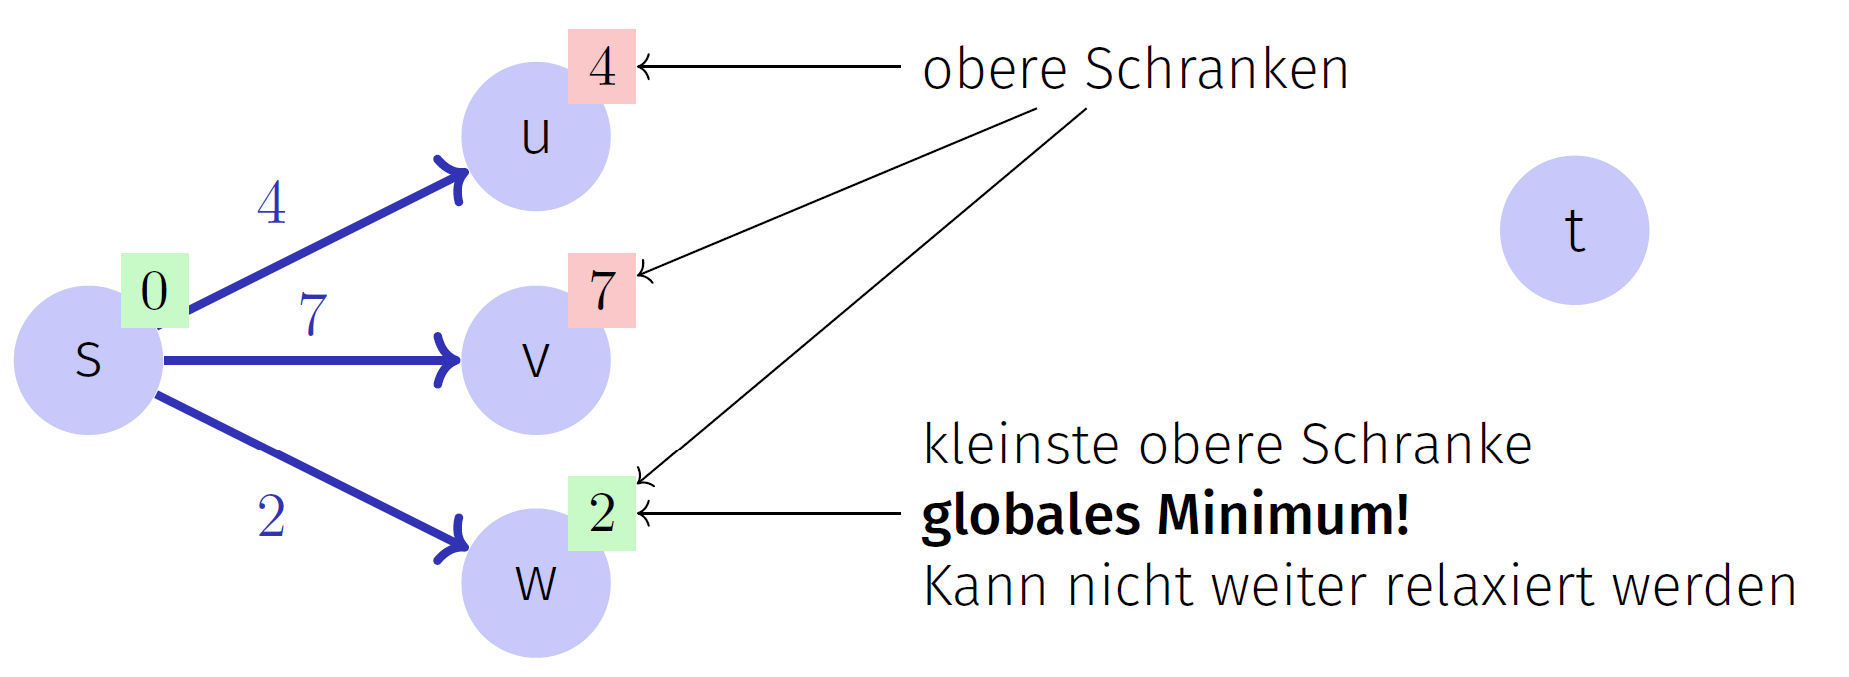
\includegraphics[width = 0.85\columnwidth]{../img/DijkstraBeobachtung.png}\par
\end{center}\smallskip

\textbf{Grundidee}\par
Menge $V$ aller Knoten wird unterteilt in
\begin{itemize}
    \item die \textcolor{red}{Menge $M$} von Knoten, für die schon ein kürzester Weg von $s$ bekannt ist
    \item die \textcolor{blue}{Menge $R=\cup_{v \in M} N^{+}(v) \backslash M$} von Knoten, für die kein kürzester Weg bekannt ist, die jedoch von $M$ direkt erreichbar sind.
    \item die \textcolor{orange}{Menge $U=V \backslash(M \cup R)$} von Knoten die noch nicht berücksichtigt wurden.
\end{itemize}

\begin{center}
    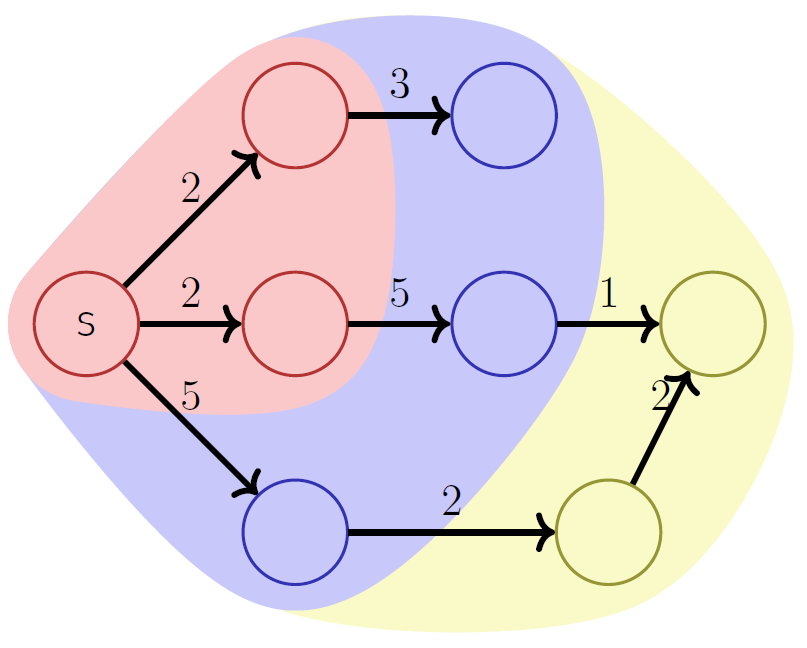
\includegraphics[width = 0.35\columnwidth]{../img/DijkstraSym.png}\par
\end{center}
\textit{Betrachte alle Nachbarn der Menge $M$ und füge den Knoten mit dem kürzesten Weg zu $s$ der Menge $M$ hinzu.}\par
\end{sectionbox}
\vspace{-4pt}
\begin{sectionbox}
\textbf{Dijkstra(G,s)}\par
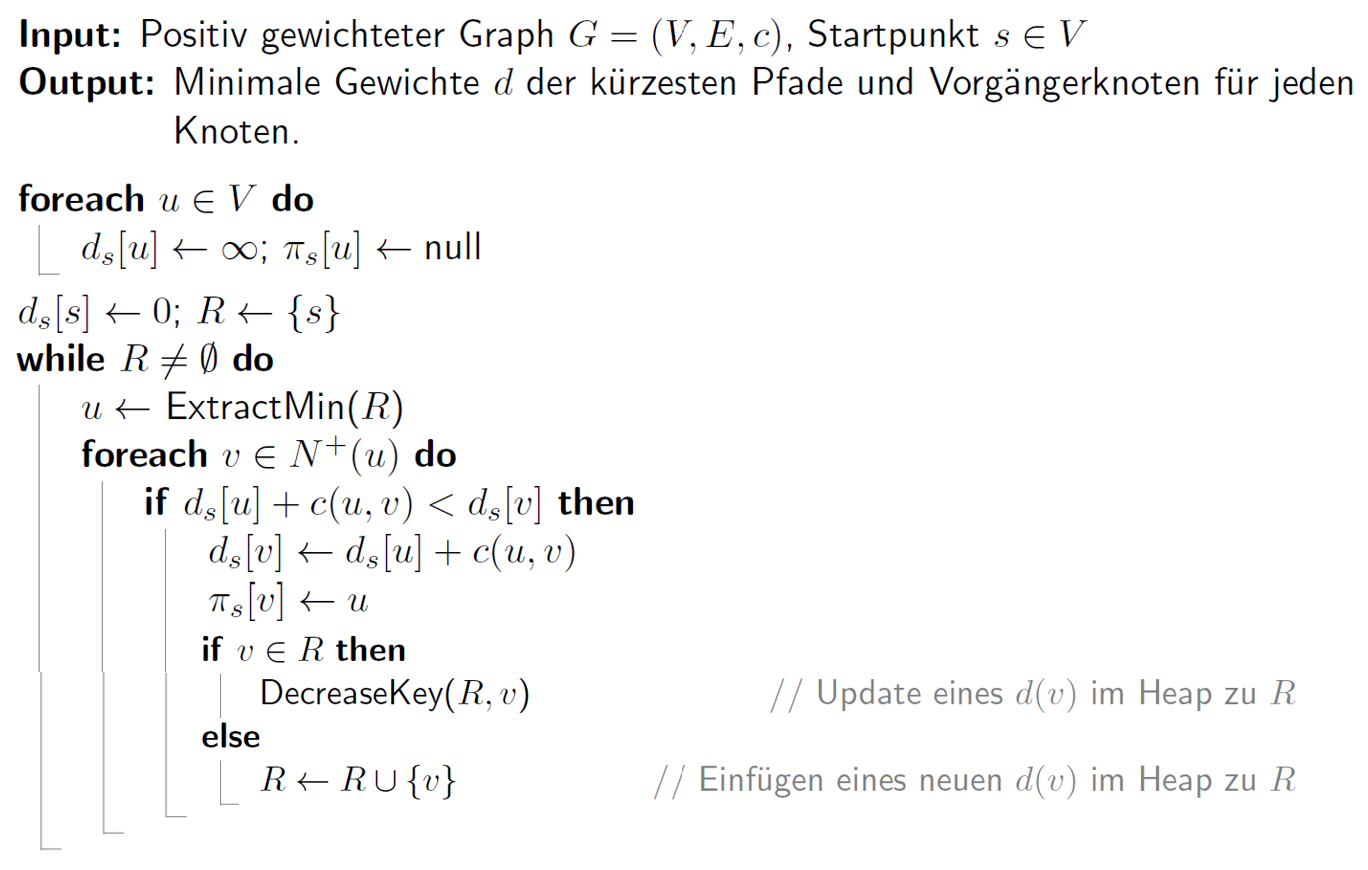
\includegraphics[width = \columnwidth]{../img/Dijkstra.png}\par
\end{sectionbox}
\vspace{-4pt}
\begin{sectionbox}
DecreaseKey (Aufsteigen im MinHeap), Position im Heap: Speichern am Knoten, Hashtabelle oder Lazy Deletion\par\smallskip
\textbf{Laufzeit}\par
\begin{itemize}
    \item $|V| \times$ ExtractMin: $\mathcal{O}(|V| \log |V|)$
    \item $|E| \times$ Insert oder DecreaseKey: $\mathcal{O}(|E| \log |V|)$
    \item $1 \times$ Init: $\mathcal{O}(|V|)$
    \item \textbf{Insgesamt}: $\mathcal{O}((|E| + |V|)\log |V|)$
\end{itemize}

\end{sectionbox}
\vspace{-4pt}
\begin{sectionbox}
\textit{Beispiel Dijkstra}\par
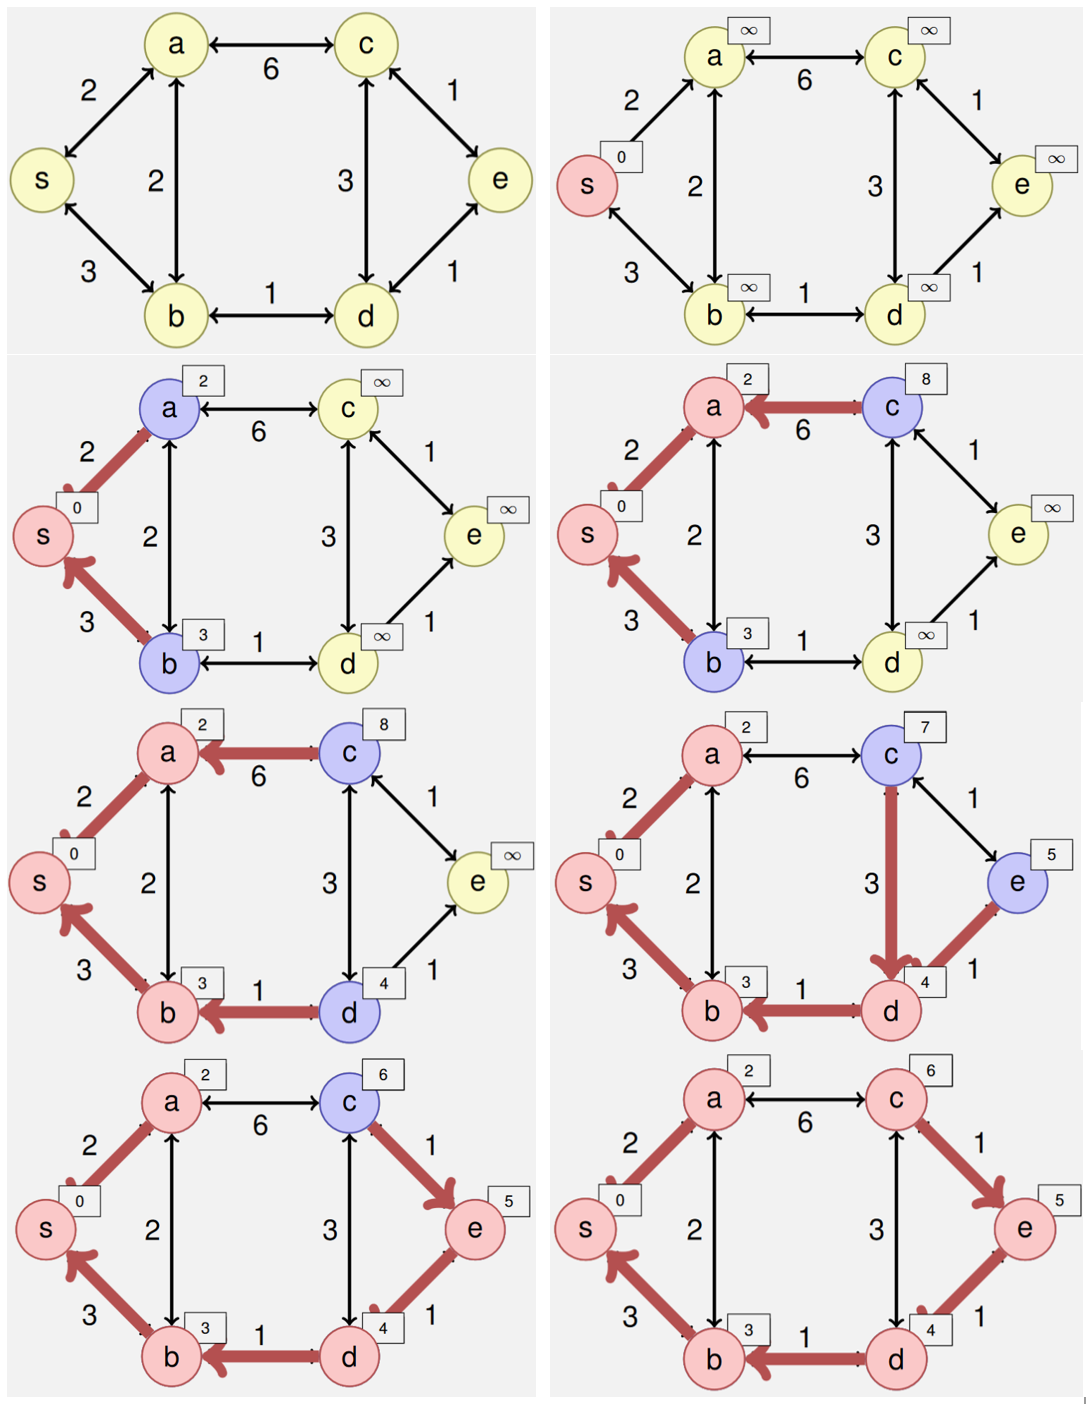
\includegraphics[width = \columnwidth]{../img/DijkstraBsp.png}\par
\end{sectionbox}

\vspace{-4pt}
\begin{sectionbox}
\subsection{Floyd-Warshall-Algorithmus}
\begin{center}
    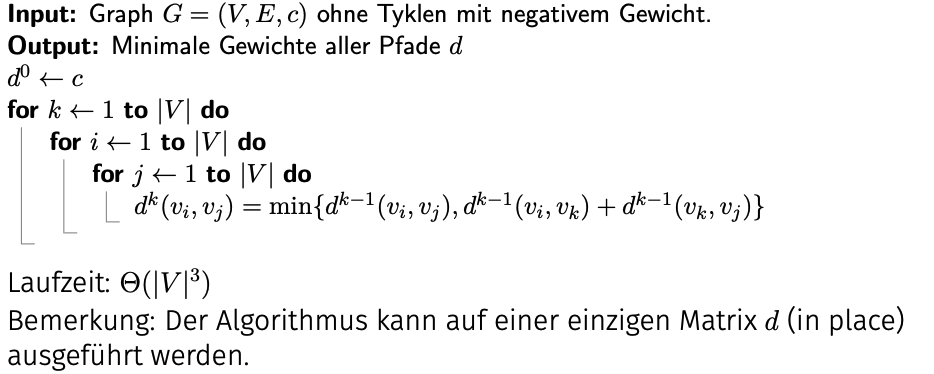
\includegraphics[width=\columnwidth]{img/FloydWarshall.png}
\end{center}
\end{sectionbox}
\vspace{-4pt}
\begin{sectionbox}
\subsection{A*-Algorithmus}
\textbf{Idee}: Abstandsheuristik $\hat{h}$ lenkt Algorithmus in richtige Richtung. Diese Heuristik muss den echten Abstand zu $t$ unterschätzen und zum
Abstand $d_s$ addiert: $f = \hat{h} + d_s$


\textbf{Voraussetzungen}
\begin{itemize}
    \item Positiv gewichteter endlicher Graph $G = (V, E, c)$
    \item $s \in V, t \in V$
    \item Absstandschätzung: $\hat{h}_t(v) \leq h_t(v) := \delta(v,t) \quad \forall v \in V$
    \item Gesucht: kürzester Pfad: $P \: : \: s \rightarrow t$
\end{itemize}

\textbf{Bemerkungen}
\begin{itemize}
    \item Mehrfaches Entnehmen \& Einfügen von $R$ beim A*-Algorithmus möglich $\Rightarrow$ Eventuell suboptimales Laufzeitverhalten
    \item Falls $\hat{h}$ zulässig $\left( \hat{h}(v) \leq h(v() \forall v \ in V)\right)$ und zusätzliche monoton $\left( \hat{h}(v) \leq h(v) + c(u',u) \forall (u',u) \in E \right)$ ist, entsprich A* dem Dijkstra-Algorithmus mit $\tilde{c} = c(u,v) + \hat{h}(u) - \hat{h}(v)$, dann wird das mehrfache einfügen in $R$ vermieden.
\end{itemize}
\end{sectionbox}
\vspace{-4pt}
\begin{sectionbox}
\textbf{A*-Algorithmus($G, s, t, \hat{h}$)}
\begin{center}
    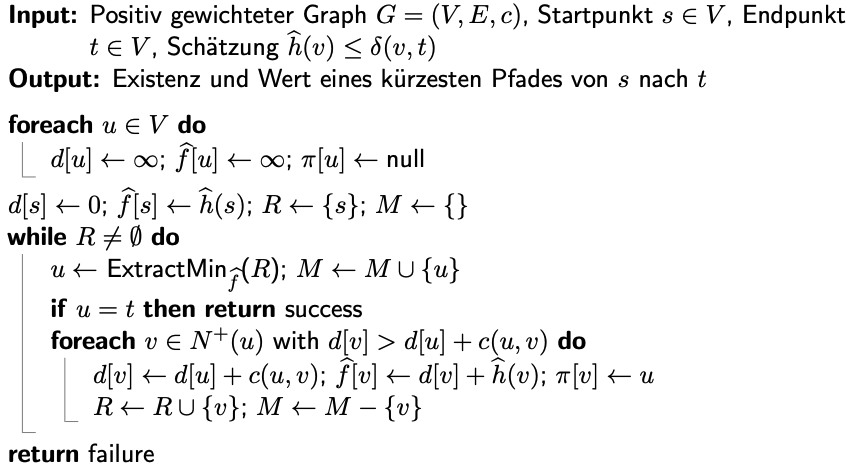
\includegraphics[width=\columnwidth]{img/AStar.png}
\end{center}

\end{sectionbox}
\vspace{-4pt}
\begin{sectionbox}
\subsection{Minimale Spannbäume}\smallskip
\textbf{Problem}\par
\begin{itemize}
    \item Gegeben: Ungerichteter, zusammenhängender, gewichteter Graph $G=(V, E, c)$
    \item Gesucht: Minimaler Spannbaum $T=\left(V, E^{\prime}\right)$ : zusammenhängender, zyklenfreier Teilgraph $E^{\prime} \subset E,$ so dass $\sum_{e \in E^{\prime}} c(e)$ minimal.
\end{itemize}
Greedy (gierige) Verfahren berechnen eine Lösung schrittweise, indem lokal beste Lösungen gewählt werden.\par
\end{sectionbox}
\vspace{-4pt}
\begin{sectionbox}
\subsubsection{Union-Find Kruskal Algorithmus}\smallskip
\textbf{Zur Implementation}\par
Gegeben eine Menge von Mengen $i \equiv A_{i} \subset V$. Zur Identifikation von Schnitten und Kreisen: Zugehörigkeit der beiden Endpunkte einer Kante zu einer der Mengen.\par
\begin{center}
    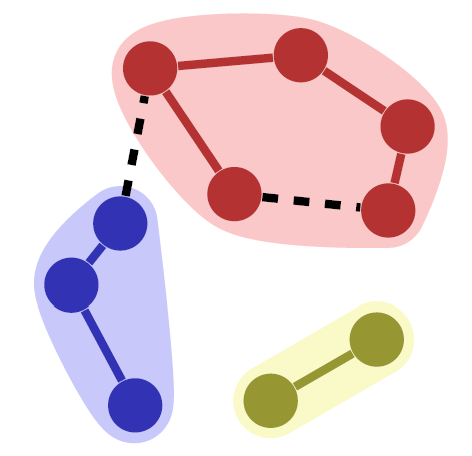
\includegraphics[width = 0.35\columnwidth]{../img/MST_Sym.png}\par
\end{center}\smallskip

Allgemeines Problem: Partition (Menge von Teilmengen) benötigt einen abstrakter Datentyp (\textbf{Union-Find}) mit folgenden Operationen:\par
\begin{itemize}
    \item Make-Set($(i)$): Hinzufügen einer neuen Menge $i$\par($p[i] \leftarrow i; return i$)
    \item Find ($e$): Name $i$ der Menge, welche $e$ enthält \par($\operatorname{while} (p[i]\neq 0) do\ i \leftarrow p[i]$; return $i$)
    \item Union($i,j$): Vereingung der Mengen mit Namen $i$ und $j$ \par($p[j]=i$, wobei $i$ und $j$ die Wurzeln (Namen) sind.)
\end{itemize}\smallskip
Laufzeitoptimierungen:\par
\begin{itemize}
    \item[a)] Immer kleineren Baum an grösseren hängen
    \item[b)] Bei Find Knoten immer an den Parent hängen
\end{itemize}\par\smallskip

\textit{Implementation von Union-Find}\par
Idee: Baum für jede Teilmenge in der Partition, z.B. {{1, 2, 3, 9}, {7, 6, 4}, {5, 8}, {10}}, wobei die Baumwurzeln $\to$ Namen (Stellvertreter) der Mengen ist.\par\smallskip
\begin{center}
    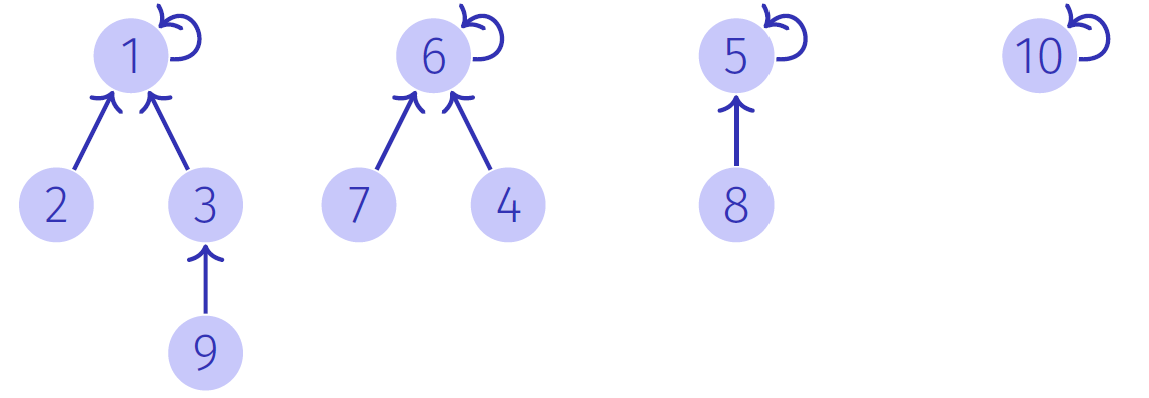
\includegraphics[width = 0.7\columnwidth]{../img/UF.png}\par\smallskip
    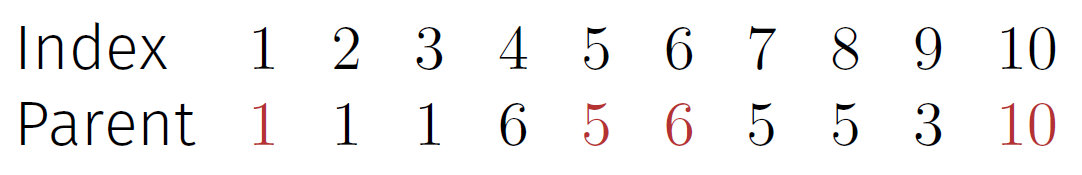
\includegraphics[width = 0.7\columnwidth]{../img/UFarray.png}\par\smallskip
\end{center}
\end{sectionbox}
\vspace{-4pt}
\begin{sectionbox}
\textbf{Algorithmus}\par
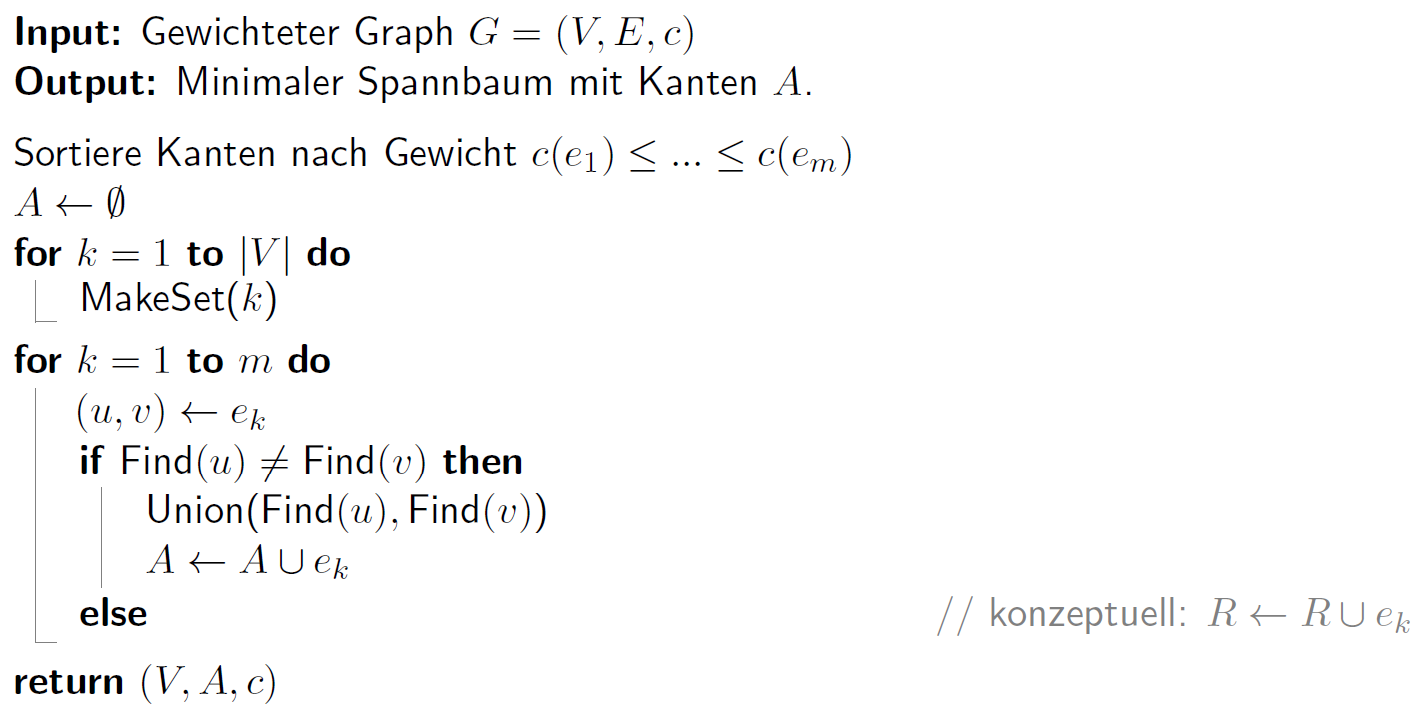
\includegraphics[width = \columnwidth]{../img/Kruskal.png}\par\smallskip

\textbf{Laufzeit des Kruskal Alghorithmus}\par
\begin{itemize}
    \item Sortieren der Kanten: $\Theta(|E| \log |E|)=\Theta(|E| \log |V|)$
    \item Initialisieren der Union-Find Datenstruktur $\Theta(|V|)$
    \item $|E| \times \text { Union }(\text { Find }(x), \text { Find }(y)): \mathcal{O}(|E| \log |V|)$
    \item \textbf{Insgesamt}: $\Theta(|E| \log |V|)$
\end{itemize}
\end{sectionbox}
\vspace{-4pt}
\begin{sectionbox}
\subsubsection{Algorithmus von Jarnik, Prim, Dijkstra}\smallskip
Idee: Starte mit einem $v \in V$ und lasse von dort unter Verwendung der Auswahlregel einen Spannbaum wachsen:\par
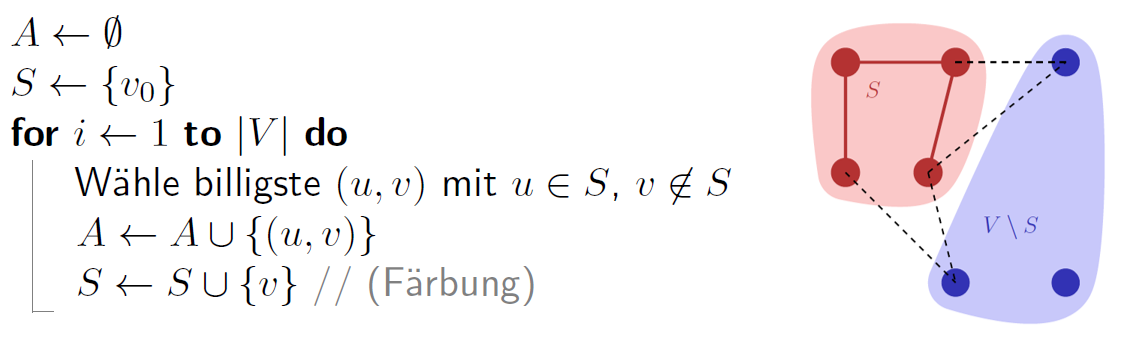
\includegraphics[width = 0.9\columnwidth]{../img/MST_JPD.png}\par\smallskip
\textit{Bemerkungen}\par
\begin{itemize}
    \item Man braucht keine Union-Find Datenstruktur (Färbung reicht aus)
    \item Vorgehensweise:
    \par \tab a) Immer Knoten mit kleinstem Gewicht zur Menge S hinzufügen
    \par \tab b) Wenn der Knoten noch nicht in S ist $\to$ MST ist zyklenfrei
\end{itemize}\par\smallskip
\textbf{Laufzeit insgesamt}: $\mathcal{O}(|E| \log |V|)$
\end{sectionbox}